\documentclass[xcolor=x11names,compress]{beamer}

%% General document %%%%%%%%%%%%%%%%%%%%%%%%%%%%%%%%%%
\PassOptionsToPackage{table}{xcolor}
\usepackage{graphicx}
\usepackage{multirow,multicol}
\usepackage{amsmath}
\usepackage{mathpazo}
\usepackage{amsthm}
\usepackage{amssymb}
\usepackage{setspace}
\usepackage{hyperref}
\usepackage{array,colortbl,booktabs}
\usepackage{soul}
\usepackage{enumerate}
\usepackage{url}
\usepackage{verbatimbox}
\usepackage{fancyvrb}
\usepackage{dirtree}
\usepackage{tikz}
\usepackage[utf8]{inputenc}
\usepackage[T1]{fontenc}
\usetikzlibrary{positioning,shapes.misc}
\usetikzlibrary{decorations.fractals}
\usetikzlibrary{calc}
\usepackage[normalem]{ulem}
\useunder{\uline}{\ul}{}
\usetikzlibrary{arrows}
\usetikzlibrary{fit}
%\usepackage{color, colortbl}
\usepackage{etoolbox}
\makeatletter
\patchcmd{\slideentry}{\advance\beamer@xpos by1\relax}{}{}{}
\def\beamer@subsectionentry#1#2#3#4#5{\advance\beamer@xpos by1\relax}%
\makeatother
%%%%%%%%%%%%%%%%%%%%%%%%%%%%%%%%%%%%%%%%%%%%%%%%%%%%%%


%% Beamer Layout %%%%%%%%%%%%%%%%%%%%%%%%%%%%%%%%%%
\useoutertheme[subsection=false, shadow]{miniframes}
\useinnertheme{circles}
\usefonttheme{structurebold}
\usepackage{palatino}
\usepackage{tcolorbox}
\usepackage{lipsum}

%% COLOR DEFINITION %%%%%%%%%%%%%%%%%%%%%%%%%%%%%%%%
\definecolor{mygold}{RGB}{236,208,120}
\definecolor{brick}{RGB}{217,91,67}
\definecolor{myred}{RGB}{192,41,66}
\definecolor{redwine}{RGB}{102,0,102}
\definecolor{myaqua}{RGB}{83,119,122}

%%%%%%%%%%%%%%%%%%%%%%%%%%%%%%%%%%%%%%%%%%%%%%%%%%%%%%

%%% OTHER EXTRA STUFF%%%%%%%%%%%%%%%%%%%%%%%%%%%%%%%%
%% CHANGE COVER SLIDE %%
\makeatletter
    \newenvironment{coverframe}{
\setbeamercolor*{palette tertiary}{fg=myaqua,bg=myaqua} 
}
    {}
\makeatother

%% CHANGE COLOR OF BULLETS %%
\setbeamercolor{item}{fg=brick} % color of bullets
\setbeamercolor{subitem}{fg=mygold}

%% DEFINE TIKZ ITEMS %%
\tikzset{
    %Define standard arrow tip
    >=stealth',
    %Define style for boxes
    punkt/.style={
           rectangle,
           rounded corners,
           draw=black, very thick,
           text width=3em,
           minimum height=2em,
           text centered},
    % Define arrow style 1
    pil/.style={
           <-,
           thick,
           shorten <=2pt,
           shorten >=2pt,}
        % Define arrow style
           }
           
 %% Perpendiculas symbol
 \newcommand\independent{\protect\mathpalette{\protect\independenT}{\perp}}
\def\independenT#1#2{\mathrel{\rlap{$#1#2$}\mkern2mu{#1#2}}}

\newcommand{\ds}{\displaystyle}

\newcommand{\bv}{\begin{Verbatim}[numbers=left, baselinestretch=1,
    xleftmargin=.5in, xrightmargin=.1in, frame=single,
    rulecolor=\color{gray}]}

%%%%%%%%%%%%%%%%%%%%%%%%%%%%%%%%%%%%%%%%%%%%%%%%%%
\setbeamerfont{title like}{shape=\scshape}
\setbeamerfont{frametitle}{shape=\scshape}
\setbeamercolor{frametitle}{fg=myaqua!120,bg=white}
\setbeamercolor{title}{fg=myaqua!120}
%\setbeamertemplate{frametitle}{\vspace{6em}}

\setbeamercolor*{lower separation line head}{bg=redwine} 
\setbeamercolor*{normal text}{fg=black} 
\setbeamercolor*{alerted text}{fg=myred} 
\setbeamercolor*{example text}{fg=brick} 
\setbeamercolor*{structure}{fg=black} 
 
\setbeamercolor*{palette tertiary}{fg=black!80,bg=white} 
\setbeamercolor*{palette quaternary}{fg=black,bg=black!10} 

\renewcommand{\(}{\begin{columns}}
\renewcommand{\)}{\end{columns}}
\newcommand{\<}[1]{\begin{column}{#1}}
\renewcommand{\>}{\end{column}}

%%%%%%%%%%%%%%%%%%%%%%%%%%%%%%%%%%%%%%%%%%%%%%%%%%
\title[Errors, Exceptions and Testing]{Python Class 3: Errors, Exceptions and Testing}
\author{Michelle Torres}
\date{August 11, 2016}

\begin{document}
\newcommand<>{\highlighton}[1]{%
  \alt#2{\structure{#1}}{{#1}}
}

\newcommand{\icon}[1]{\pgfimage[height=1em]{#1}}

%%%%%%%%%%%%%%%%%%%%%%%%%%%%%%%%%%%%%%%%%%%%%%%%%%
%%%%%%%%%%%%%%%%%%%%%%%%%%%%%%%%%%%%%%%%%%%%%%%%%%
%%%%%%%% START THE SLIDES %%%%%%%%%%%%%%%%%%%%%%%%
%%%%%%%%%%%%%%%%%%%%%%%%%%%%%%%%%%%%%%%%%%%%%%%%%%
%%%%%%%%%%%%%%%%%%%%%%%%%%%%%%%%%%%%%%%%%%%%%%%%%%

\begin{coverframe}
\begin{frame}
\titlepage	
\end{frame}
\end{coverframe}


\section[Outline]{}
\frame{\tableofcontents}

\section{Errors}
\begin{frame}[fragile]
  \frametitle{Types of Errors}
  \begin{itemize}
  	  \item \textcolor{redwine}{Syntax error}
	  \begin{itemize}
		  \item Errors related to language structure. 
		  \item Forgotten symbols, types, or confusing object names.
		  \item Check the \^{}!
	  \end{itemize} 
\begin{small}
	\begin{Verbatim}[commandchars=\\\{\}]
>>> while True print 'Hello world' \pause
>>> while True print \textcolor{red}{:} 'Hello world'\pause
>>> class = "Advanced Computronics for Beginners" 
Traceback (most recent call last):
  In line 1 of the code you submitted:
    class = "Advanced Computronics for Beginners"
          ^
SyntaxError: invalid syntax
\end{Verbatim}
\end{small}
\end{itemize}
\end{frame}

\begin{frame}[fragile]
\begin{itemize}
	\item \textcolor{redwine}{Runtime error}
  \begin{itemize}
  	\item Errors during the execution of program. 
	\item eg. TypeError, NameError, ZeroDivisionError \pause
 \end{itemize}
 \begin{footnotesize}
  \begin{Verbatim}[commandchars=\\\{\}]
>>> callMe = "Maybe"
>>> print(callme)
Traceback (most recent call last):
  In line 2 of the code you submitted:
    print(callme)
\textcolor{red}{NameError}: name 'callme' is not defined \pause
>>> print("you cannot add text and numbers" + 12)
Traceback (most recent call last):
  In line 1 of the code you submitted:
    print("you cannot add text and numbers" + 12)
\textcolor{red}{TypeError}: Can't convert 'int' object to str implicitly
\end{Verbatim}	
 \end{footnotesize}
 \end{itemize}
\end{frame}

\frame{
A \textcolor{redwine}{syntax error} happens when Python can't understand what you are saying. A \textcolor{myaqua}{run-time error} happens when Python understands what you are saying, but runs into trouble when following your instructions.\\\

In English, a \textcolor{redwine}{syntax error} would be like the sentence:

\begin{center}
\textit{Please cat dog monkey.}	
\end{center}

The grammar of this sentence does not make sense!\\\

In English, a \textcolor{myaqua}{run-time error} would be like the sentence:
\begin{center}
	\textit{Please eat the piano.}
\end{center}
}

\begin{frame}[fragile]
\begin{itemize}
  \item \textcolor{myred}{Semantic error}
  \begin{itemize}[<+->]
  	\item The program will run successfully but the output is not what you expect.
  	\item Task: create a program that calculates the average of two numbers ($\frac{x+y}{2}$)
  	
  	\begin{verbatim}
>>>  x = 3
>>>  y = 4
>>>	 average = x + y / 2
>>>	 print(average)

5.0 # ????
  	\end{verbatim}
  	\item Very common, very annoying and, unfortunately, without indication that they exist.
	\item My deep and thoughtful advice: Debug, debug, debug! Test, test, test!
 \end{itemize}
  \end{itemize}
\end{frame}

\begin{frame}[fragile]
\frametitle{Debugging Tips}
Make sure:
\begin{itemize}
\item You are not using a reserved/keyword. 

\begin{verbatim}
>>> import keyword
>>> keyword.kwlist
\end{verbatim}

\pause

\item You have \textcolor{red}{:} after \texttt{for}, \texttt{while}, etc. \pause

\item Parentheses and quotations are closed properly. \pause

\item You use = and == correctly. \pause

\begin{footnotesize}
\begin{verbatim}
>>>  x=1
>>>  if(x=1): print x
  File "<ipython-input-9-24daa00946ff>", line 1
    if(x=1): print x
        ^
SyntaxError: invalid syntax
\end{verbatim}
	
\end{footnotesize}

\item Indentation is correct! Remember, even spaces in empty lines count.
\end{itemize}
\end{frame}

\section{Exceptions}

\frame{
\frametitle{Exceptions}
\begin{small}
\begin{itemize}
\item \texttt{raise: \#to create exceptions or errors} \pause

\item \texttt{pass \#to continue execution without doing anything} \pause

\item \texttt{try: \#tries executing the following} \pause

\ \ \ ....

\texttt{except TypeError: }

\ \ \ ... \texttt{\# runs if a Type Error was raised}

\texttt{except:}

\ \ \ ... \texttt{\# runs for other errors or exceptions}

\texttt{else:}

\ \ \  ... \texttt{\# runs if there was no exception/error}

\texttt{finally:}

\ \ \ ... \texttt{\# always runs!}

\pause

\item You can create your own exceptions using classes. \pause
\item Some examples: \texttt{InClass03.py}
\end{itemize}	
\end{small}
}

%\begin{frame}
%\frametitle{Exceptions vs. Errors}%
%	An \textcolor{myred}{Error} indicates serious problems that a reasonable application should not try to catch.\\\

%An \textcolor{mygold}{Exception} indicates conditions that a reasonable application might want to catch.
%\end{frame}


\section{Testing}


\frame{
\frametitle{Unit Testing}

\begin{itemize}
\item Write tests before or as you write code. \pause

\item Test the smallest possible \emph{unit}. \pause

\item Automate tests. \pause

\item Test-driven development.

\end{itemize}

}


\frame{
\frametitle{Why Unit Test?}

\begin{itemize}
\item Find bugs quickly. \pause

\item Forces code structure. \pause

\item Allows easier integration of multiple functions. \pause

\item Much easier to return to code.
\begin{itemize}
\item Write a test for what you want to implement next. \pause
\end{itemize}

\item Easier to make code changes.
\item You can easily incorporate lots of these into your work flow.  
\end{itemize}
}

\frame{
\frametitle{Sample Test}
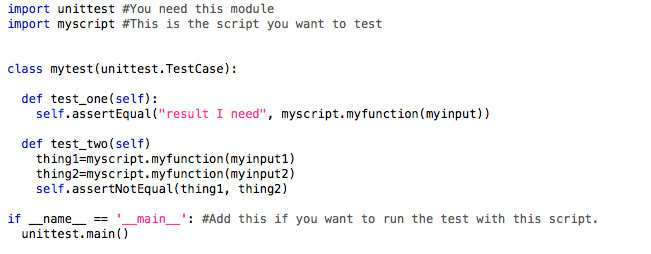
\includegraphics[width=\textwidth]{sampletest}
}

\frame{
\frametitle{Test Functions}
\begin{itemize}
\item \texttt{self.assertEqual(,)} \pause
\item \texttt{self.assertNotEqual(,)} \pause
\item \texttt{self.assertTrue(,)} \pause
\item \texttt{self.assertFalse(,)} \pause
\item \texttt{self.assertRaises(,)} \pause
\end{itemize}

Useful link: \url{https://docs.python.org/2/library/unittest.html}

}

\begin{frame}[fragile]
\begin{scriptsize}
	\begin{verbatim}
import unittest

class TestStringMethods(unittest.TestCase):

    def test_upper(self):
        self.assertEqual('foo'.upper(), 'FOO')

    def test_isupper(self):
        self.assertTrue('FOO'.isupper())
        self.assertFalse('Foo'.isupper())

    def test_split(self):
        s = 'hello world'
        self.assertEqual(s.split(), ['hello', 'world'])
        # check that s.split fails when the separator is not a string
        with self.assertRaises(TypeError):
            s.split(2)

if __name__ == '__main__':
    unittest.main()
	\end{verbatim}	
\end{scriptsize}
\end{frame}

\section{Break, Continue and Else}

\begin{frame}[fragile]
\frametitle{Break, Continue and Else}
\begin{itemize}
\item These statements can be handy using \texttt{while} or \texttt{for} loops. \pause
\item \texttt{break \#stops the loop} \pause
\item \texttt{continue \# moves on to the next iteration} \pause
\item \texttt{else \#executed only if all iterations are completed} \pause
\end{itemize}
\begin{verbatim}
>>> for n in range(2, 10):
...     for x in range(2, n):
...         if n % x == 0:
...             print(n, 'equals', x, '*', n//x)
...             break
...     else:
...         print(n, 'is a prime number')
...
\end{verbatim}
\end{frame}

\end{document}
